\section{A machine model for line-rate routers}
\label{s:absmachine}
\begin{figure}[!t]
  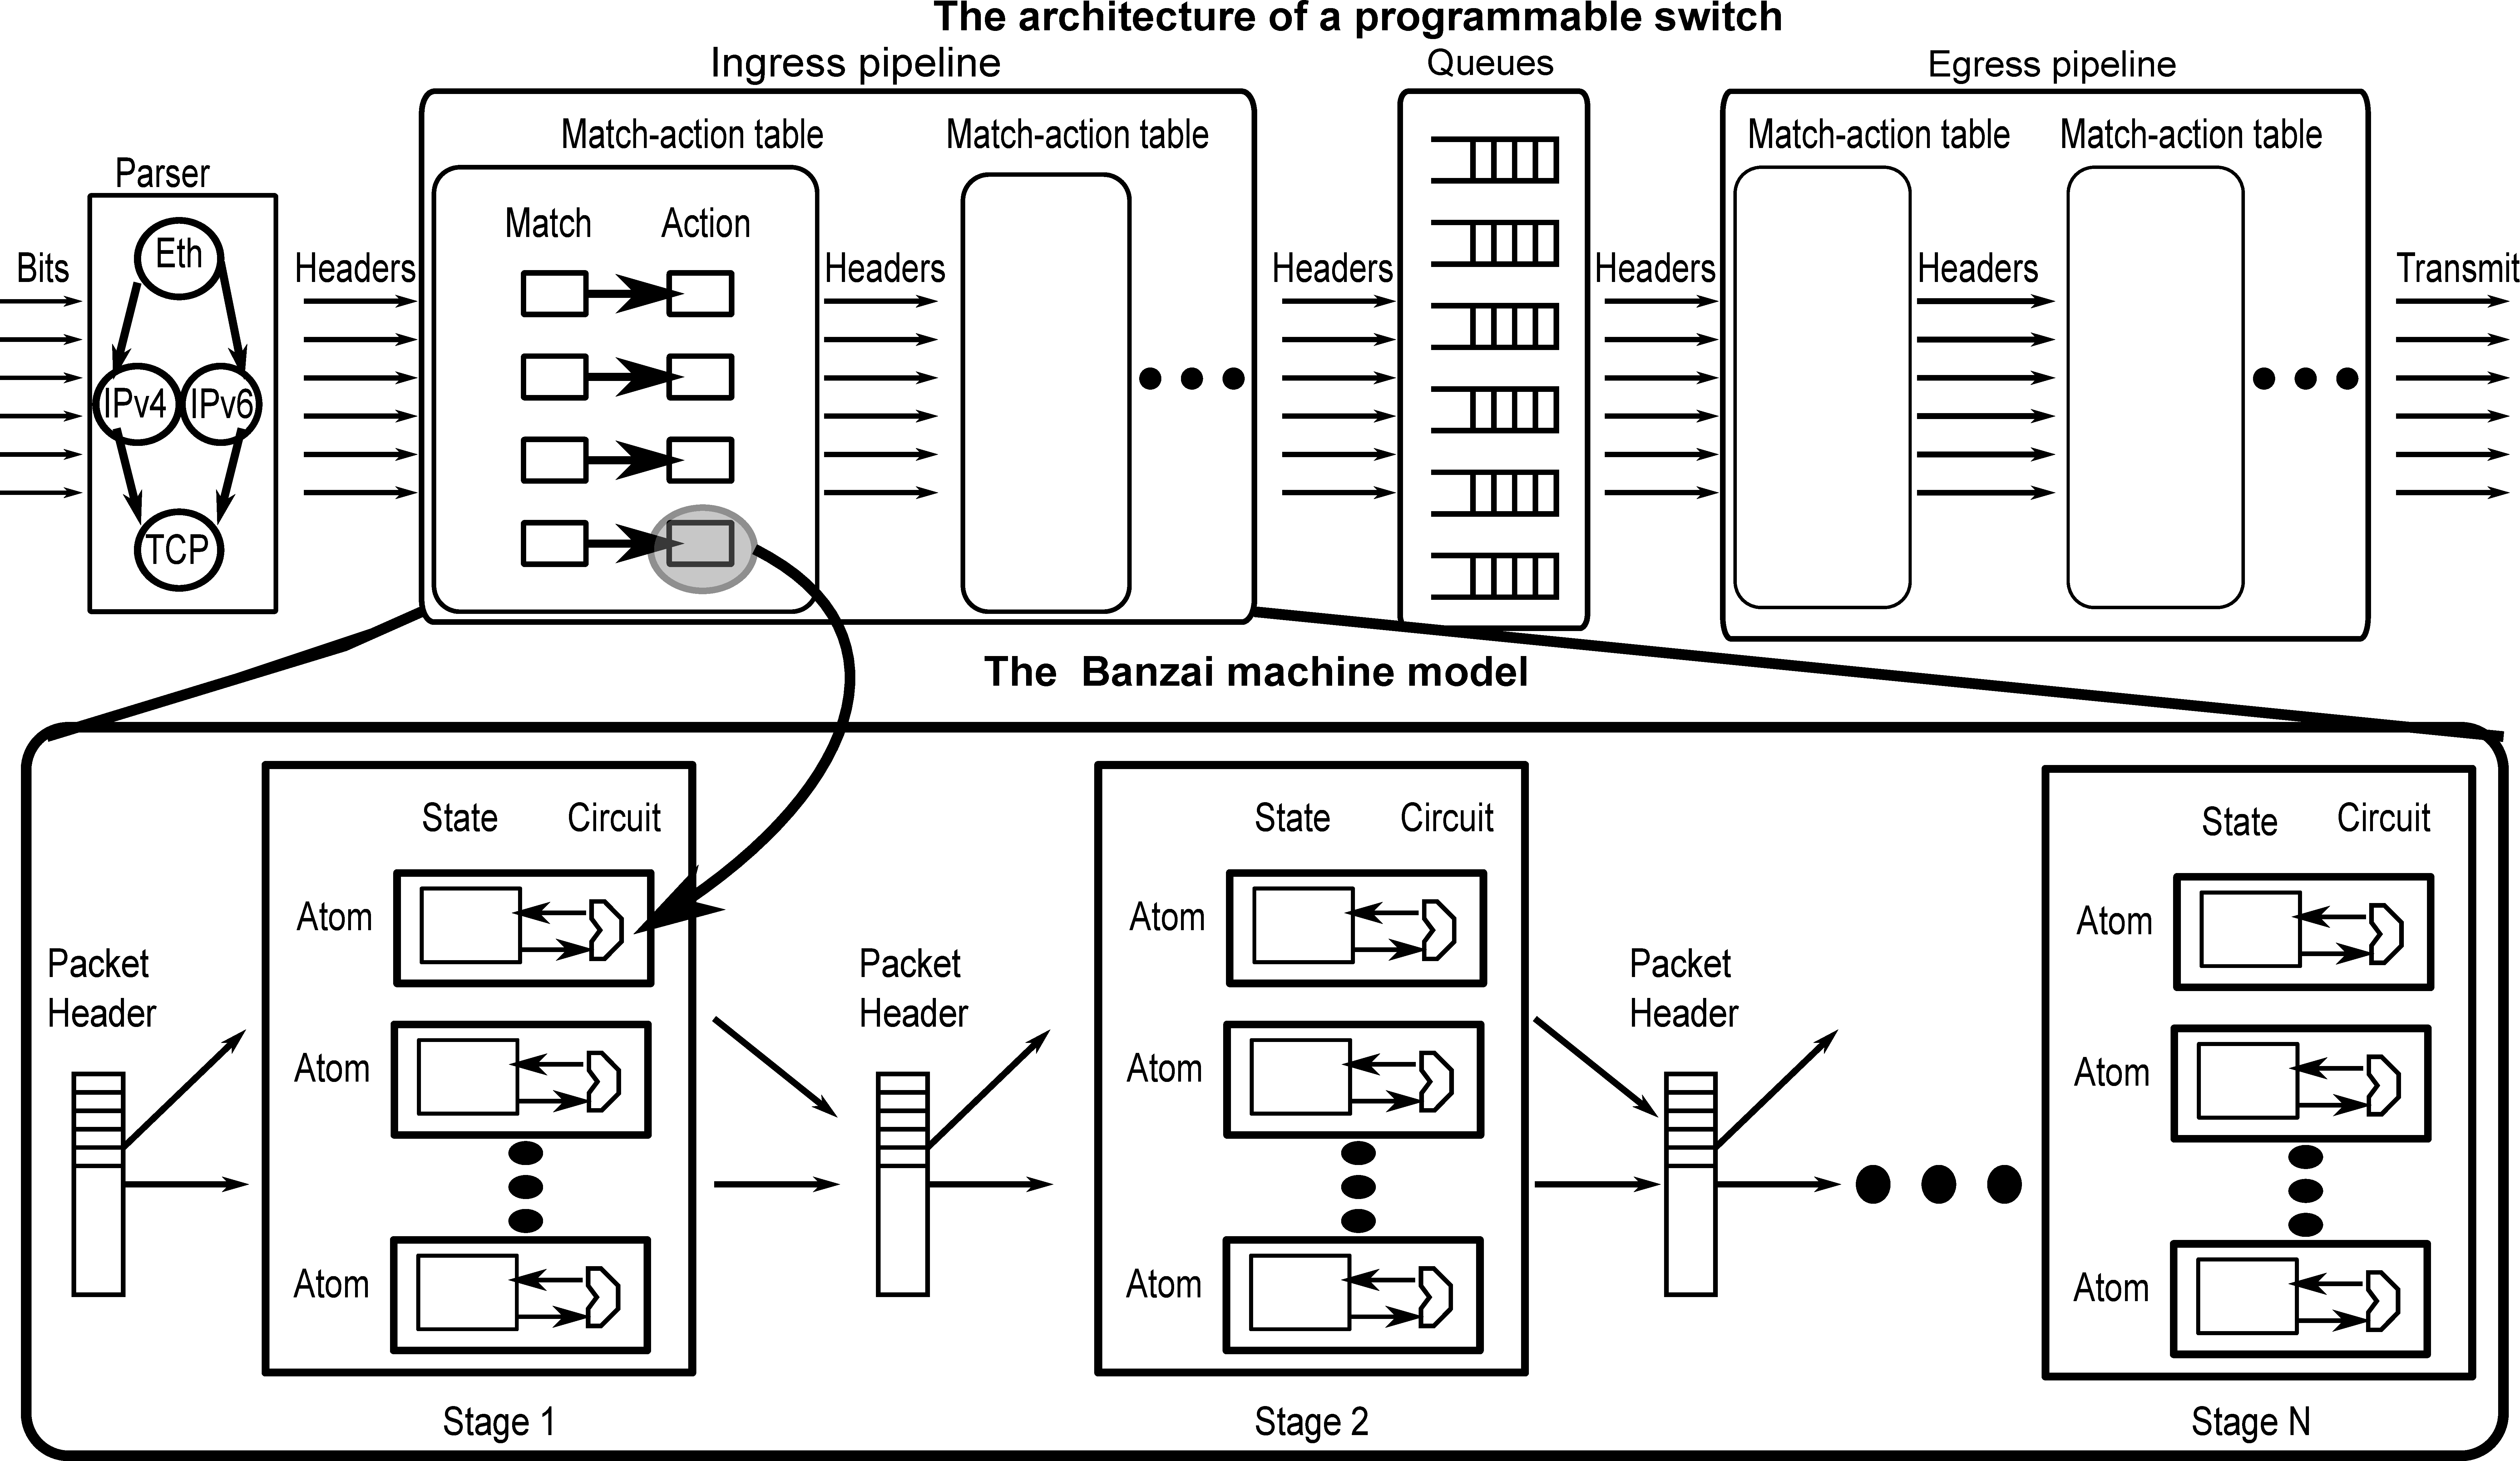
\includegraphics[width=\textwidth]{domino_banzai.pdf}
  \caption{\absmachine models the ingress or egress pipeline of a
  programmable router. An atom corresponds to an action in a match-action
  table. Internally, an atom contains local state and a digital circuit 
  modifying this state. Figure~\ref{fig:atom} details an atom.}
  \label{domino_fig:router}
\end{figure}

\absmachine is a machine model for programmable line-rate routers that serves
as the compiler target for \pktlanguage.  \absmachine is inspired by recent
programmable router architectures such as Barefoot Networks'
Tofino~\cite{tofino}, Intel's FlexPipe~\cite{flexpipe}, and Cavium's XPliant
Packet Architecture~\cite{xpliant}. \absmachine abstracts these architectures
and extends them with stateful processing units to implement data-plane
algorithms.  These processing units, called {\em atoms}, model atomic
operations that are supported by a programmable line-rate router and serve as
the instruction set of the router.

\subsection{Background: programmable routers}
Packets arriving at a router~(top half of Figure~\ref{domino_fig:router}) are
parsed by a programmable parser that turns packets into header fields. These
header fields are first processed by an ingress pipeline consisting of
match-action tables arranged in stages. Processing a packet at a stage may
modify its header fields, through match-action rules, as well as some
persistent state at that stage, \eg packet counters. After the ingress
pipeline, the packet is queued. Once the scheduler dequeues the packet, it is
processed by a similar egress pipeline before it is transmitted.

%TODO: Don't say there's only a single pipeline
To reduce chip area, each ingress and egress pipeline is shared across a number
of router ports and handles aggregate traffic belonging to all these ports,
regardless of packet sizes. The number of ingress and egress pipelines depends
on the aggregate capacity of the router. For instance, a 64-port router with a
line rate of 10 Gbit/s per port and a minimum packet size of 64 bytes needs to
process around a billion packets per second, after accounting for minimum
inter-packet gaps~\cite{rmt}.  This requirement can be supported by a single
pipeline that runs at 1 GHz.  For higher aggregate capacities, multiple 1-GHz
pipelines are required.\footnote{It is technically challenging to achieve a
clock rate higher than 1 GHz in router ASICs.} Throughout this chapter, we
assume a single pipeline router, with the pipeline running at 1 GHz.
Equivalently, every pipeline stage handles a new packet every clock cycle (1
ns).
%TODO: Add a section on multiple pipelines later.

Having to process a packet every clock cycle in each stage constrains the
operations that can be performed on each packet. In particular, any packet
operation that modifies state visible to the next packet {\em must} finish
execution in a single clock cycle (\S\ref{ss:atoms} shows why). Because of this
restriction, any programmable router chip will have to provide a small set of
processing units or primitives for manipulating packets and state in a stage,
unlike a software router. These primitives determine which algorithms can run
on the router at line rate.

The challenge for us is to develop primitives that allow a broad range of
data-plane algorithms to be implemented, and to build a compiler to map a
user-friendly description of an algorithm to the primitives provided by a
router.

\subsection{The \absmachine machine model}

\absmachine (the bottom half of Figure~\ref{domino_fig:router}) models the
ingress or egress router pipeline.  It models the computation within a
match-action table in a stage (\ie the action half of the match-action table),
but not how packets are matched (\eg direct or ternary). \absmachine does not
model packet parsing and assumes that packets arriving to \absmachine are
already parsed.
%We discuss how to embed \absmachine in a standard match-action
%pipeline in \S\ref{ss:guards}.  

 Concretely, \absmachine is a feed-forward pipeline\footnote{It is hard to
physically route backward-flowing wires that would be required for feedback.}
consisting of a number of stages executing synchronously on every clock cycle.
Each stage processes one packet every clock cycle and hands it off to the next.
Unlike a CPU pipeline, which occasionally experiences pipeline stalls,
\absmachine's pipeline is deterministic, never stalls, and always sustains line
rate. However, relative to a CPU pipeline, \absmachine is restricted in the
operations it supports (\S\ref{s:atomConstraints}).

\subsection{Atoms: \absmachine's processing units}
\label{ss:atoms}
 An {\em atom} is an atomic unit of packet processing supported natively by a
\absmachine machine, and the atoms within a \absmachine machine form its
instruction set. Each pipeline stage in \absmachine contains a vector of atoms.
Atoms in this vector modify mutually exclusive sections of the same packet
header in parallel in every clock cycle, and process a new packet header every
clock cycle.
%TODO: Clear up latency vs. throughput distinction here.

In addition to packet headers, atoms may modify persistent state on the router
to implement stateful data-plane algorithms. To support such algorithms at
line-rate, the atoms for a \absmachine machine need to be substantially richer
(Table~\ref{tab:templates}) than the simple RISC-like stateless instruction
sets for programmable routers~\cite{rmt}. We explain why below.

Suppose we need to atomically increment a router counter to count packets. One
approach is hardware support for three simple RISC-like single-cycle
operations: (1) \textit{read} the counter from memory in the first clock cycle,
(2) \textit{add} one in the next, and (3) \textit{write} it to memory in the
third.  This approach, however, does not provide atomicity. To see why, suppose
packet $A$ increments the counter from 0 to 1 by executing its read, add, and
write at clock cycles 1, 2, and 3 respectively.  If packet $B$ issues its read
at time 2, it will increment the counter again from 0 to 1, when it should be
incremented to 2.

Locks over the shared counter are a potential solution.  However, locking
causes packet $B$ to wait during packet $A$'s increment, and the router no
longer sustains the line rate of one packet every clock cycle. CPUs employ
micro-architectural techniques such as operand forwarding for this problem. But
these techniques still suffer pipeline stalls, which prevents line-rate
performance from being achieved. Instead, \absmachine's approach to resolving
this problem is to provide a small set of atomic operations and reject programs
that require anything else because line-rate performance cannot be guaranteed
for them.

For instance, in the case of the counter, \absmachine provides an atomic
increment operation at line rate with an {\em atom} to read a counter,
increment it, and write it back in a single stage within one clock cycle. It
uses the same approach of reading, modifying, and writing back to implement
other stateful atomic operations at line rate.

Unlike stateful atomic operations, stateless atomic operations are easier to
support with simple packet-field arithmetic.  Consider, for instance, the
operation {\tt pkt.f1 = pkt.f2 + pkt.f3 - pkt.f4}.  This operation does not
modify any persistent router state and only accesses packet fields. It can be
implemented atomically by using two atoms: one atom to add fields f2 and f3 in
one pipeline stage, and another to subtract f4 from the result in the next. An
instruction set designer can provide {\em simple} stateless instructions
operating on a pair of packet fields. These instructions can then be composed
into larger stateless operations, without designing atoms specifically for each
stateless operation.

\medskip
\noindent
\textbf{Representing atoms.}
An atom is represented by a body of sequential code that captures the atom's
behavior. It may also contain internal state local to the atom. An atom
completes execution of this entire body of code, modifying a packet and any
internal state before processing the next packet. The designer of a
programmable router would develop these atoms, and expose them to a router
compiler as the programmable router's instruction set, \eg
Table~\ref{tab:templates}.

Using this representation, a router counter that wraps around at a
value of 100 can be written as the atom:\footnote{We use {\tt p.x} to
  represent field {\tt x} within a packet {\tt p} and {\tt x} to
  represent a state variable {\tt x} that persists across packets.}
\begin{lstlisting}[style=customc, numbers=none, frame=none]
if (counter < 99)
  counter++;
else
  counter = 0;
\end{lstlisting}

Similarly, a stateless operation like setting a packet field to a constant
value can be written as the atom:
\begin{lstlisting}[style=customc, numbers=none, frame=none]
  pkt.field = value;
\end{lstlisting}

\subsection{Constraints for line-rate operation}
\label{s:atomConstraints}

\medskip
\noindent
\textbf{Memory limits.} State in \absmachine is local to each atom.  It can
neither be shared by atoms within a stage, nor by atoms across stages. This is
because building multi-ported memories (to store the state) accessible to
multiple atoms is technically challenging and consumes additional chip area.
However, state can be read into a packet header in one stage, for subsequent
use by a downstream stage\footnote{Figure~\ref{fig:flowlet_pipeline} shows an
example. {\tt last\_time} is read into {\tt pkt.last\_time} in stage 2, for
subsequent use by stage 3.}.  But, the \absmachine pipeline is feed-forward, so
state can only be carried forward, not backward.

\medskip
\noindent
\textbf{Computational limits.} Atoms need to execute atomically from one packet
to the next, so any state internal to the atom must be updated before the next
packet arrives.  Because packets may be separated by as little as one clock
cycle, we mandate that atom bodies finish execution within one clock cycle, and
constrain atom bodies to do so.

We constrain atom bodies by defining {\it atom templates}
(\S\ref{ss:code_gen}).  An atom template is a program with configurable
parameters that terminates within a clock cycle and specifies the atom's
behavior.  An example is an ALU with a restricted set of primitive operations
(Figure~\ref{fig:alu_diag}).

% Atom templates allow us to create
%and experiment with \absmachine machines with different atoms.

%As programmable
%routers evolve, we expect that atoms will evolve as well, but constrained by
%the clock-cycle requirement.

\begin{figure}[h]
  \begin{subfigure}{0.5\columnwidth}
  \centering
  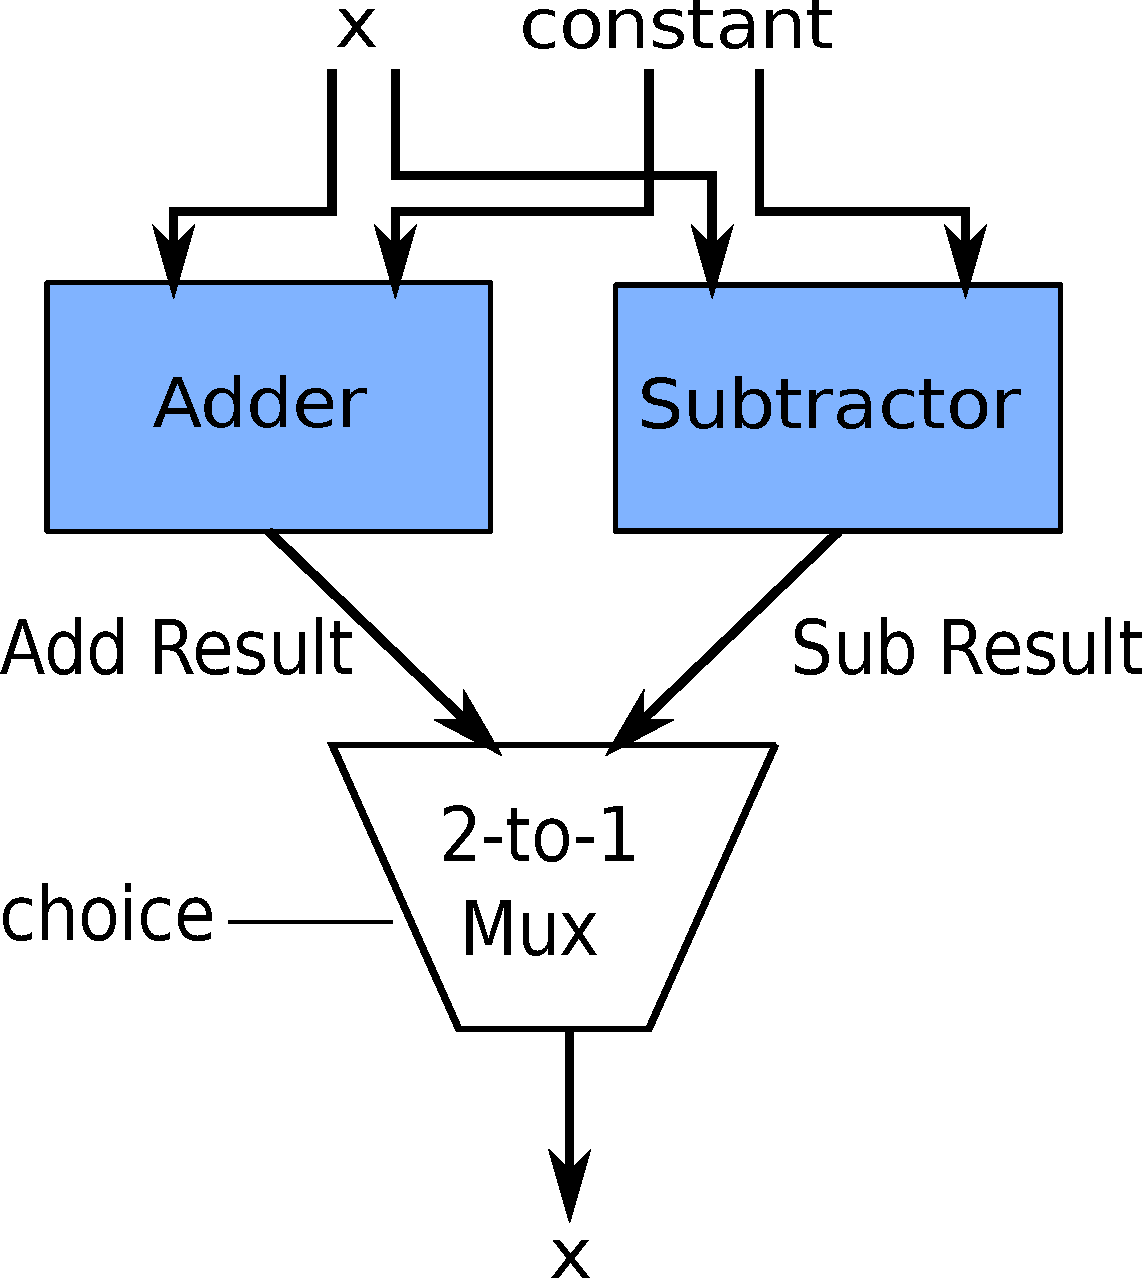
\includegraphics[width=0.5\textwidth]{domino_circuit.pdf}
  \caption{Circuit for the atom}
  \label{fig:alu_diag}
  \end{subfigure}
  \hspace{0.1\columnwidth}
  \begin{subfigure}{0.3\columnwidth}
  \begin{lstlisting}[belowskip=-0.8 \baselineskip]
  bit choice = ??;
  int constant = ??;
  if (choice) {
    x = x + constant;
  } else {
    x = x - constant;
  }
  \end{lstlisting}
  \hspace{0.1\columnwidth}
  \caption{Atom template}
  %Each ``??(n)'' represents a hole that can be filled in with values in $[0, 2^n -1]$.}
  \label{fig:alu_in_sketch}
  \end{subfigure}
  \caption{An atom and its template. The atom above can add or subtract a constant from a state
  variable {\tt x} based on two configurable parameters, {\tt constant} and {\tt choice}.}
  \label{fig:atom}
\end{figure}

\medskip
\noindent
\textbf{Resource limits.} We also limit the number of atoms in each stage
(\textit{pipeline width}) and the number of stages in the pipeline
(\textit{pipeline depth}). This is similar to limits on the number of stages,
tables per stage, and memory per stage in programmable router
architectures~\cite{lavanya_compiler}.

\subsection{What can \absmachine not do?}
\label{domino_ss:limitations}

\absmachine is a good fit for data-plane algorithms that modify a small set of
packet headers and carry out small amounts of computation per packet.
Data-plane algorithms like deep packet inspection and WAN optimization require
a router to parse and process the packet payload as well---effectively parsing
a large ``header'' consisting of each byte in the payload. This is challenging
at line rates of 1 GHz, and such algorithms are best left to CPUs~\cite{e2}.
Some algorithms require complex computations, but not on every packet, \eg a
measurement algorithm that periodically scans a large table to perform garbage
collection.  \absmachine's atoms model small operations that occur on every
packet, and are unsuitable for such operations that span many clock cycles.
